\begin{flushright} {\tiny {\color{gray} \tt supg.tex}} \end{flushright}
%------------------------------------------------------------------------------

As abundantly documented in the literature advection needs to be stabilised
as it otherwise showcases non-negligible under- and overshoots.
A standard approach is the Streamline Upwind Petrov Galerkin (SUPG) 
method\footnote{Note that \textcite{mayu91} (1991) speak of ``streamwise-upwinding Petrov-Galerkin'' method}.

A nice overview of upwind techniques and how SUPG came to be is to be found in Chapter 
2 of \textcite{dohu03} or in \textcite{brhu82}.
\textcite{humm86} (1986) present a review of the SUPG method 
and discuss an additional discontinuity-capturing term. 
So do \textcite{tepa86} (1986).
Note that the idea of upwind goes back to the seventies, see for example 
\textcite{hehz77} (1977).

It is compared to other methods in the context of mantle convection in 
Malevsky \& Yuen (1991) \cite{mayu91} (rotating cone, convection in a box). 
Note that SUPG is not restricted to advection(-diffusion) equations: it can also
be applied to the Navier-Stokes equations\footnote{\url{https://en.wikipedia.org/wiki/Streamline_upwind_Petrov-Galerkin_pressure-stabilizing_Petrov-Galerkin_formulation_for_incompressible_Navier-Stokes_equations}}

As explained in the step-9 tutorial of deal.II (\url{https://www.dealii.org/current/doxygen/deal.II/step_9.html}), the term `Petrov-Galerkin' can be explained as follows: 
\begin{displayquote}
{\color{MidnightBlue}
A ``Galerkin method'' is one where one obtains the weak formulation by multiplying the equation by a test function $v$ (and then integrating over $\Omega$) where the functions $v$ are from the same space as the solution $u$ (though possibly with different boundary values). But this is not strictly necessary: One could also imagine choosing the test functions from a different set of functions, as long as that different set has ``as many dimensions'' as the original set of functions so that we end up with as many independent equations as there are degrees of freedom (where all of this needs to be appropriately defined in the infinite-dimensional case). Methods that make use of this possibility (i.e., choose the set of test functions differently than the set of solutions) are called ``Petrov-Galerkin'' methods. }
\end{displayquote}

%------------------------------
\subsection{The SUPG method}

We start from the 'bare-bones' heat transport equation (source terms are omitted): 
\begin{equation}
\rho C_p \left( \frac{\partial T}{\partial t} + {\vec \upnu}\cdot {\vec\nabla T} \right)
= {\vec \nabla} \cdot (k \vec\nabla T )
\end{equation}
which we once again write 
\begin{equation}
\rho C_p \left(\dot{T} + {\vec \upnu}\cdot {\vec\nabla T} \right)
= {\vec \nabla} \cdot (k \vec\nabla T )
\end{equation}

In what follows we assume that the velocity vield $\vec \upnu$ is known so that temperature is the
only unknown.
Let $\bN^\uptheta_i$ be the temperature basis function at node $i$ so that the temperature inside an element is
given by\footnote{the $\uptheta$ superscript has been chosen to denote temperature so as to avoid confusion
with the transpose operator}:
\begin{equation}
T^h({\vec r}) = \sum_{i=1}^{m_T} \bN^\uptheta_i ({\vec r})\;  T_i = \vec \bN^\uptheta \cdot \vec T
\end{equation}
where $\vec T$ and $\vec \bN^\uptheta$ are vectors of length $m_T$. Also, in 2d:
\[
\vec \nabla \vec \bN^\uptheta = 
\left(
\begin{array}{cccc}
\partial_x \bN_1^\uptheta & 
\partial_x \bN_2^\uptheta & \dots &
\partial_x \bN_{m_T}^\uptheta \\ \\
\partial_y \bN_1^\uptheta & 
\partial_y \bN_2^\uptheta & \dots &
\partial_y \bN_{m_T}^\uptheta 
\end{array}
\right)
\]
The weak form is then of the form
\begin{equation}
\int_{\Omega_e} \bN^\uptheta_i \left[ 
\rho C_p \left( \dot{T} + {\vec \upnu}\cdot {\vec\nabla T} \right) \right] d\Omega
= \int_{\Omega_e}  \bN^\uptheta_i {\vec \nabla} \cdot (k \vec\nabla T ) d\Omega
\end{equation}
or, rather we look for the discrete temperature $T^h$ such that
\[
\underbrace{\int_{\Omega_e} \bN^\uptheta_i  \rho C_p \dot{T}^h d\Omega}_{I}
+ \underbrace{\int_{\Omega_e} \bN^\uptheta_i  \rho C_p  {\vec \upnu}\cdot {\vec\nabla T^h}   d\Omega}_{II}
= \underbrace{\int_{\Omega_e}  \bN^\uptheta_i {\vec \nabla} \cdot (k \vec\nabla T^h )d\Omega}_{III}
\quad\quad
i=1,m_T
\]
We have already worked out in Section~\ref{ss:hte_fem} the terms $I$, $II$ and $III$.
The streamline upwind Petrov-Galerkin (SUPG) 
method adds the following stabilisation term to the left hand side of this equation (see Section 2.4 
in \textcite{dohu03}):
\begin{equation}
\int_{\Omega_e} (\vec\upnu\cdot\vec\nabla \bN_i^\theta ) \tau {\cal R}(T^h,\vec\upnu) \; d\Omega
\label{eq:supg:res1}
\end{equation}
where ${\cal R}$ is the residual defined as
\begin{equation}
{\cal R}(T^h,\vec\upnu) = 
\rho C_p (\dot{T}^h +  {\vec \upnu}\cdot {\vec\nabla T^h}) - {\vec \nabla} \cdot k \vec\nabla T^h 
\label{eq:supg:res2}
\end{equation}
and $\tau$ is a stabilization parameter (see Section~\ref{ss:tausupg}).

Since $I$, $II$ and $III$ have been worked out already, 
we here after only focus on the additional SUPG terms. 
  
Given Eq.~\eqref{eq:supg:res1} and \eqref{eq:supg:res2} we then have three terms to deal with:
\begin{eqnarray}
IV &=&\int_{\Omega_e} \tau(\vec\upnu\cdot\nabla \bN_i^\theta) (\rho C_p\dot{T}^h)  d\Omega \\
V  &=&\int_{\Omega_e} \tau(\vec\upnu\cdot\nabla \bN_i^\theta)(\rho C_p{\vec \upnu}\cdot{\vec\nabla T^h}) d\Omega \\
VI &=&\int_{\Omega_e} \tau(\vec\upnu\cdot\nabla \bN_i^\theta)(-{\vec \nabla} \cdot k \vec\nabla T^h ) d\Omega 
\end{eqnarray}
and we must solve $I + II + IV + V + VI = III$. 
We can compute the quantities $I+IV$, $II+V$ and $III-VI$:
\begin{eqnarray}
I+IV 
&=&
\int_{\Omega_e} \bN^\uptheta_i  \rho C_p \dot{T}^h d\Omega 
+
\int_{\Omega_e}(\vec\upnu\cdot\vec\nabla \bN_i^\theta)  \tau ( \rho C_p\dot{T}^h)  d\Omega \nn\\
&=& 
\int_{\Omega_e} ( \bN^\uptheta_i + \tau \vec\upnu\cdot\vec\nabla \bN_i^\theta )  ( \rho C_p\dot{T}^h)  d\Omega 
\\
II+V 
&=&
\int_{\Omega_e} \bN^\uptheta_i  \rho C_p  {\vec \upnu}\cdot {\vec\nabla T^h}   d\Omega
+
\int_{\Omega_e}(\vec\upnu\cdot\vec\nabla \bN_i^\theta) \tau (\rho C_p {\vec \upnu}\cdot{\vec\nabla T^h}) d\Omega \nn\\
&=& 
\int_{\Omega_e} (\bN^\uptheta_i  + \tau \vec\upnu\cdot\vec\nabla \bN_i^\theta) (\rho C_p {\vec \upnu}\cdot{\vec\nabla T^h}) d\Omega \\
III- VI &=& \int_{\Omega_e}  \bN^\uptheta_i {\vec \nabla} \cdot (k \vec\nabla T^h )d\Omega
- \int_{\Omega_e} \tau(\vec\upnu\cdot\nabla \bN_i^\theta)(-{\vec \nabla} \cdot k \vec\nabla T^h ) d\Omega \nn\\
&=& \int_{\Omega_e}  (\bN^\uptheta_i    + \tau \vec\upnu\cdot\vec\nabla \bN_i^\theta) {\vec \nabla}    \cdot (k \vec\nabla T^h )d\Omega
\end{eqnarray}



\begin{remark}
If the equation is a pure advection equation, then the heat conductivity $k=0$ so $III=VI=0$. 
\end{remark}


We see that both $I+IV$ and $II+V$ contain the term $\bN^\uptheta_i  + \tau \vec\upnu\cdot\vec\nabla \bN_i^\theta$
which we can interpret as a 'modified' basis function:
\[
\boxed{
\underline{\bN}^\uptheta_i = \bN^\uptheta_i  + \tau \vec\upnu\cdot\vec\nabla \bN_i^\theta
}
\]
This yields the following modified elemental matrices
\begin{eqnarray}
{\M}^\uptheta \quad &\rightarrow& \quad \underline{\M}^\uptheta
= \int_{\Omega_e} \rho C_p \vec{\underline{\bN}}^\uptheta \vec{\bN}^\uptheta \; d\Omega
\\
{\K}_a \quad &\rightarrow & \quad \underline{\K}_a 
= \int_{\Omega_e} \rho C_p \vec{\underline{\bN}}^\uptheta ({\vec \upnu}\cdot \vec\nabla \vec{\bN}^\uptheta) \; d\Omega
\\
{\K}_d \quad &\rightarrow&  \quad \underline{\K}_d 
=\int_{\Omega_e} k \vec\nabla \vec{\underline{\bN}}^\uptheta \cdot \vec\nabla \vec{\bN}^\uptheta d\Omega
\end{eqnarray}


These notations may look attractive but the modified diffusion matrix contains the gradient 
of the modified basis functions and working this out in practice proves to be cumbersome and 
not practical for higher order basis functions. Also the surface term arising from the integration by parts 
containing these modified basis functions might lose its physical significance. 
As such, we will therefore keep $\K_d$ (coming from the integration by parts of $III$, and 
its associated surface flux term not shown above) and $VI$ separated. 

Under the assumption that $k$ is constant within the element $\Omega_e$, we have 
\[
VI = \int_{\Omega_e} \tau(\vec\upnu\cdot\nabla \bN_i^\theta)(- k \Delta T^h ) d\Omega 
\]
with 
\[
\Delta T^h 
= \Delta \left( \sum_{i=1}^{m_T} \bN^\uptheta_i ({\vec r}) T_i \right)
= \sum_{i=1}^{m_T} \Delta \bN^\uptheta_i ({\vec r}) T_i 
= \Delta \vec \bN^\uptheta \cdot \vec T
\]
If the basis functions are first-order ones, then $VI=0$ since $\Delta \vec \bN^\uptheta = \vec 0$.  



\begin{remark} 
The modified mass matrix is not symmetric anymore. 
This is not necessarily problematic since the 
advection matrix is also not symmetric so that the solver of choice for the equation already can 
deal with such matrices.
\end{remark} 


The SUPG-stabilised pure advection equation is extensively tested in \stone~43.


%---------------------------------------------------------------------------
\subsection{About the choice of the parameter $\tau$}\label{ss:tausupg}

\begin{enumerate}
\item The approach used in step-63 and subsequently in \aspect{} is the 
one in John \& Knobloch \cite{jokn06,knob08} which is also to be found in early 
80's papers \cite{brhu82,hubr82}:
\[
\tau_1 = \frac{h}{2 |\vec\upnu| p} \left( \coth (\Penb) - \frac{1}{\Penb} \right)
\qquad
\Penb = \frac{|\vec\upnu| h}{2 \kappa p}
\]
where $\tau$ is computed on each cell, $h$ being its diameter in the direction of $\vec\upnu$, 
and $p$ is the order of the approximation (i.e. the maximum degree of polynomials).

\begin{center}
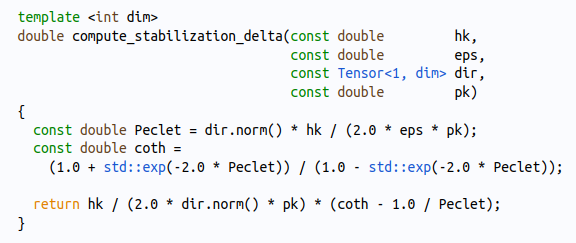
\includegraphics[width=9cm]{images/supg/step63}\\
{\captionfont Taken from step-63 webpage 
at \url{https://www.dealii.org/current/doxygen/deal.II/step_63.html}}
\end{center}

A quick note about 
\[
\beta(x) = \coth (x) -\frac{1}{x}
\]
If $x\rightarrow \infty$ then $1/x \rightarrow 0$ and then
\[
\beta(x) \rightarrow \coth(x) 
= \frac{\exp(x) + \exp(-x)}{\exp(x)-\exp(-x)}
= \frac{1 + \exp(-2x)}{1-\exp(-2x)} \rightarrow 1
\]
If $x \rightarrow 0$ then we must use the Taylor expansion of the $\exp$ function:
\[
\exp(x) \simeq 1 +x +x\frac{x^2}{2} + \frac{x^3}{6}
\]
Then 
\begin{eqnarray}
\exp(x) + \exp(-x)
&\simeq& 1 +x +\frac{x^2}{2} + \frac{x^3}{6} + ...
+ 1 -x +\frac{x^2}{2} - \frac{x^3}{6} + ...
\simeq 2 + x^2 \nn\\
\exp(x) - \exp(-x) 
&\simeq& 1 +x +\frac{x^2}{2} + \frac{x^3}{6} + ...
- 1 +x -\frac{x^2}{2} + \frac{x^3}{6} + ...
\simeq 2x 
\end{eqnarray}
so that 
\[
\beta(x) \rightarrow \frac{2+x^2}{2x} - \frac{1}{x} = \frac12 x
\]
In both cases the function $\beta$ is bounded and positive. 



The expression above is also found at p. 617 in \textcite{lomw12}.
Note that Hughes \& Brooks \cite{hubr82} replace the costly '$\coth$' term by an asymptotic curve:

\begin{center}
\includegraphics[width=8cm]{images/supg/hubr82}\\
{\captionfont Taken from \textcite{hubr82} (1982). Here $\alpha$ is the Peclet number.} 
\end{center}

Note also that in \textcite{hubr82} (1982) the authors present the 
following formulation for the 2d case:
\begin{center}
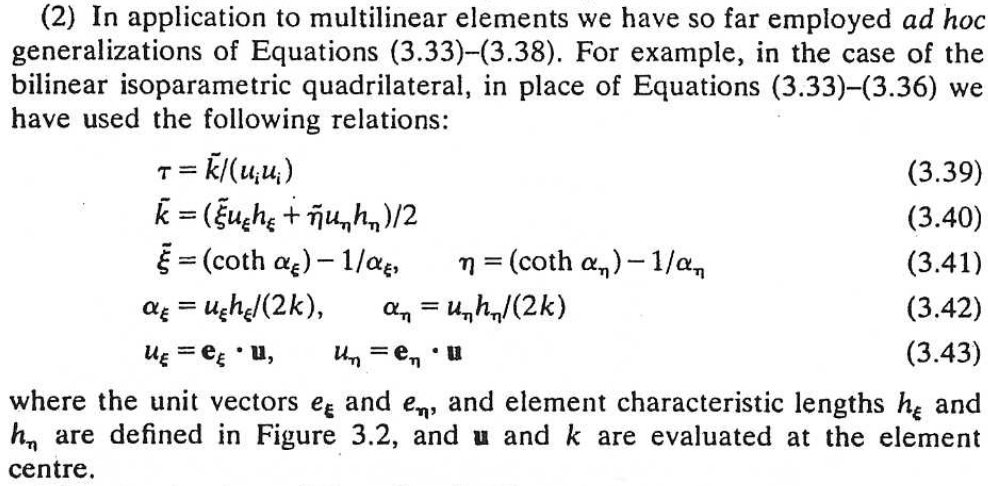
\includegraphics[width=9cm]{images/supg/hubr82b}\\
{\captionfont Taken from \textcite{hubr82} (1982).} 
\end{center}
This approach will certainly prove to be rather expensive!



\item
Codina (2000) (see Eq.39 of \cite{codi00}, see also Eq.2.64 of \textcite{dohu03}) defines $\tau$ as follows:
\[
\tau_2= \left( \frac{2 |\vec\upnu|}{h} + \frac{4 \kappa}{h^2} + \sigma   \right)^{-1}
\]
where $\sigma$ is a reaction term (which we neglect in what follows). This equation 
can be re-written:
\[
\tau_2= \frac{h}{2 |\vec\upnu|} \left( 1 + \frac{1}{\Penb} \right)^{-1}
\]



\item In \textcite{dohu03} we find the expression proposed by Shakib and co-workers (see Eq. 3.59 of \cite{shhj91}):
\[
\tau_3=\left( \left(\frac{2|\vec\upnu|}{h} \right)^2 
+9 \left(\frac{4\kappa}{h^2} \right)^2 + \sigma^2  \right)^{-1/2}
= \frac{h}{2|\vec\upnu|} \left(  1 + \frac{9}{\Penb^2} 
+ \left(\frac{h}{2|\vec\upnu|} \sigma  \right)^2 \right)^{-1/2}
\]

\item
Braun \cite{brau03} uses 
\[
\tau_4 = \frac{h}{|\vec\upnu| \sqrt{15}} = \frac{h}{2|\vec\upnu|} \frac{2}{\sqrt{15}} 
\]
This formula is independent of $\Penb$ and is also in \textcite{bogs04} (2004).
It is also used in Hughes \& Brooks (1982) \cite{hubr82} for pure advection problems in 1D
and this value is attributed to Raymond \& Garder (1976)  \cite{raga76}.

\item Following \textcite{teos00} (see also Appendix A of Thieulot (2011) \cite{thie11}):
\[
\tau_5 = \left( \frac{2 |\vec{\upnu}|}{h} + \frac{1}{\theta \delta t} + \frac{\kappa}{h^2} \right)^{-1}  
\]
Crank-Nicolson: $\theta=1/2$, CFL condition yields $\delta t = C \frac{h}{|\vec\upnu|}$ so 
\[
\tau_5 = \left( \frac{2 |\vec{\upnu}|}{h} + \frac{2}{\delta t}+  \frac{\kappa}{h^2}  \right)^{-1}  
= \left( \frac{2 |\vec{\upnu}|}{h} + \frac{2 v}{C h} +  \frac{\kappa}{h^2}  \right)^{-1}  
= \frac{h}{2 |\vec{\upnu}|}  \left( 1 + \frac{1}{C} + \frac{1}{4 \Penb} \right)^{-1} \nn 
\]
Note that the velocity in the CFL criterion is the maximum velocity in the domain, while 
in all other expressions above for $\tau_i$ it is the velocity in the cell/element. 
By doing so, the relationship  for $\tau_5$ is actually only valid for the cell with the 
highest velocity. 
Also, this has been used in the context of SUPG methods for the Navier-Stokes equations, 
not advection-diffusion equations! This approach is then not considered further.

\item \textcite{frhm04} (2004) use the following formula which originates from 
\textcite{frfh92} (1992): if $0\le \Penb < 1$ then
$\tau = \frac{h}{2 |\vec\upnu|} \Penb$ and if $\Penb \ge 1$ then $\tau = \frac{h}{2 |\vec\upnu|}$.
Note however that their definition of the Peclet number includes a scalar parameter $m$ which is 
the minimum between 1/3 and and 2$C_k$ where the calculation of this parameter is discussed in 
Remarks 4 and 5 of \cite{frfh92}. The authors conclude that for linear quadrilaterals the value
1/3 should be used while for biquadratic elements 1/12 should be preferred.
The same approach is found in \textcite{brbf92} (1992). 

\item Knobloch \cite{knob08} discusses other choices of $\tau$.


\end{enumerate}

Quoting Donea \& Huerta: "It is obvious that $\tau$ must vanish when the mesh is refined (no stabilisation
is necessary for a fine enough mesh)" and "Numerical experiments seem to indicate that for 
finite elements of order $p$ the value of the stabilisation parameter should be approximately 
$\tau/p$."

Let us define the dimensionless coefficient 
$\gamma_j=\frac{\tau_j}{h/2|\vec\upnu|}$ and 
plot this quantity against the Peclet number:

\begin{center}
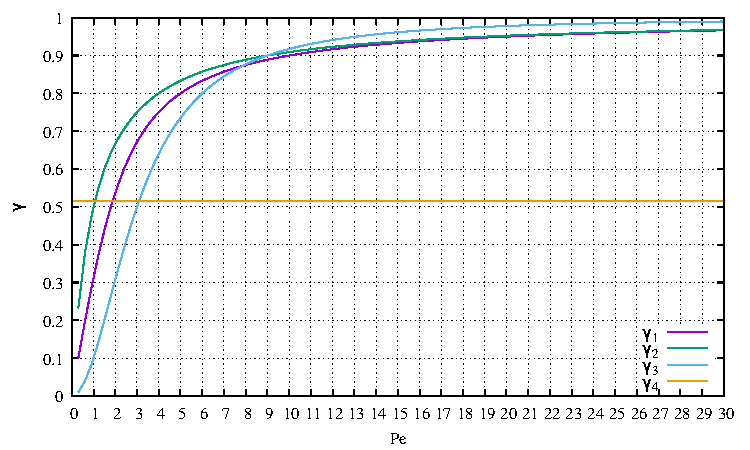
\includegraphics[width=10cm]{images/supg/gamma}\\
{\captionfont in images/supg/ folder. Note that gnuplot
struggles with small values of $\Penb$ and the purple line should 
actually reach the origin.} 
\end{center}

In the case when the equation to be stabilised is a pure advection equation, 
then $\Penb\rightarrow \infty$ so 
\[
\gamma_1 \rightarrow 1/p  \quad
\gamma_2 \rightarrow 1 \quad
\gamma_3 \rightarrow 1 \quad
\gamma_4 \simeq 0.52 \quad
\gamma_5 \rightarrow (1+C^{-1})^{-1} 
\]
Note that in most versions above (except $\tau_1$) 
$\tau$ does not depend on the order $p$ of the basis functions.
Is it an omission?

Finally it is worth mentioning that \textcite{dohu03} argue that $\tau$ should 
ideally take different values at the corners and at the mid-side nodes for quadratic elements (p.~61).

%------------------------------
\subsection{Some remarks about Appendix A of Thieulot (2011) \cite{thie11}}
\label{ss:appAthie11}

In the \douar paper \cite{brtf08} or the \fantom paper \cite{thie11},
The advection matrix is simply modified and computed as follows:
\[
({\K}_a^e)_{SUPG}
=
\int_{x_k}^{x_{k+1}}   ({\vec \bN}^\star)^T \rho C_p \vec\upnu \cdot {\bm B} dx  
\quad\quad
{\text with}
\quad\quad
{\vec \bN}^\star= {\vec \bN} + \tau \vec \upnu \cdot {\bm B}
\]
Note that we can also write 
\[
({\K}_a^e)_{SUPG}
=
\int_{x_k}^{x_{k+1}}   {\vec \bN}^T \rho C_p \vec\upnu \cdot {\bm B} dx  
+
\int_{x_k}^{x_{k+1}}  \tau (\vec \upnu \cdot {\bm B})^T   \rho C_p (\vec\upnu \cdot {\bm B}) dx  
\]
and we see that the SUPG method introduces and additional term that is akin to 
a diffusion term in the direction of the flow.
This can be seen by looking at the advection matrix a regular grid of 1D 
elements of size $h$:
\[
({\K}_a^e)_{SUPG}=
{\K}_a^e
+
\rho C_p
\frac{\tau u^2}{h}
\left(
\begin{array}{cc}
1 & -1 \\ \\
-1 & 1
\end{array}
\right)
\]
The additional matrix has the same structure as the 1D diffusion matrix matrix in \ref{sec:diff1D}.

The parameter $\tau$ is chosen as follows \cite{teos00}:
\begin{equation}
\tau= \left(\frac{1}{\tau_1} + \frac{1}{\tau_2} + \frac{1}{\tau_3} \right)^{-1}
\qquad
\tau_1=\frac{h}{2 |\vec\upnu|},
\quad
\tau_2 = \theta \; \delta t,
\quad
\tau_3 = \frac{h^2 \rho C_p}{k}
\label{tausupg}
\end{equation}
where $h$ is a measure of the element size and $\theta$ is related to the time
discretisation scheme ($\theta$ = 1/2 corresponds to a mid-point implicit scheme),
and we can define $\gamma=\tau |\vec\upnu|/h$ (see Appendix A of \cite{thie11}). 

A typical test case for testing an advection scheme is the step advection benchmark 
(see for instance Donea \& Huerta (2003) \cite{dohu03}). At $t=0$, 
a field $T(x)$ is prescribed in a 1D domain of unit length. For $x\le 1/4$ we have $T(x)=1$ and 
$T(x)=0$ everywhere else as shown on the following figure:
\begin{center}
\includegraphics[width=8cm]{images/supg/fantom3}\\
{\captionfont Taken and modified from Thieulot (2011) \cite{thie11}}
\end{center}
The prescribed velocity is $\upnu=1$, 50 elements are used ($h=0.02$) and 250 time steps are 
carried out with $\delta t=0.1h/\upnu=0.002$ (CFL number of 0.1).
Then it follows that $\tau_3=\infty$ (no diffusion, i.e. $k=0$) and 
\[
\tau
= \left(\frac{2}{0.02} + \frac{2}{0.002} \right)^{-1}
= \left(\frac{1}{0.01} + \frac{1}{0.001} \right)^{-1}
= \left(\frac{1}{0.01} (1 + \frac{1}{10})  \right)^{-1}
= 0.01 \left(\frac{11}{10}  \right)^{-1}
\simeq 0.009091
\]
which yields $\gamma = 0.00909/0.02=0.4545...$
Using this value leads to a desired removal of the oscillations through a small
amount of numerical diffusion. Braun \cite{brau03} argues for a constant
$\gamma=1/\sqrt{15}=0.258$ (citing Hughes \& Brooks (1982) \cite{hubr82}), 
which effect is also shown in the figure above. This 
value is arguably too large and introduces an undesirable diffusion. Note that this same value is 
to be found in \textcite{bogs04} (2004). The authors then state that 
"for 1D pure advection problems, this choice maximizes the phase accuracy in the semidiscrete
equation" and cite Raymond \& Gardner (1976) \cite{raga76} as source. 

Another classic example of advection testing is a 2d problem where (for example) a cylinder, a Gaussian 
and a cone are prescribed and advected with a velocity field (see for instance \cite{dohu03}). 

\begin{center}
\includegraphics[width=0.45\textwidth]{images/supg/supg1}
\includegraphics[width=0.45\textwidth]{images/supg/supg2}\\
{\captionfont After a $2\pi$ rotation and in the absence of stabilisation we see that the temperature field
showcases clearly visible ripples.}
\end{center}

\begin{remark}
Note that \aspect{} originally did not rely on the SUPG formulation to stabilise the 
advection(-diffusion) equations\cite{krhb12}. It instead relied on the Entropy Viscosity
formulation \cite{gupp10,gupp11}.
It is only during the 6th Hackathon in May 2019 that the SUPG was introduced on the code.
Note that the \aspect{} implementation is based on the deal.II step 
63\footnote{\url{https://www.dealii.org/developer/doxygen/deal.II/step_63.html}}.
\end{remark}


%-----------------------------------------------------
\subsection{A note about linear elements - artificial diffusion}

We have seen in Section~\ref{ss:femvsfdm} that the discretised advection-diffusion equation 
in 1D can be written in a manner akin to the Finite Difference method:
\[
\frac{u}{2h}
\left[
\left(1-\frac{1}{\Penb}\right) T_{i+1} + \frac{2}{\Penb} T_i - \left(1+\frac{1}{\Penb}\right)T_{i-1} 
\right] = f
\]
and we show in \stone~65 that the solution is far from accurate for $\Penb>1$ (i.e. systems where advection 
dominates over diffusion). Let us ask ourselves the 
following question: could we come up with a modified version of the equation above which 
guarantees an exact solution on a uniform mesh of linear elements?

Essentially, we are looking for $A$, $B$ and $C$ such that 
{\color{red} not sure I understand this sentence} 
\[
A T_{i+1} + BT_i + C T_{i-1} = f
\]
One can show (see Donea \& Huerta \cite{dohu03}) that a successful 
candidate formulation is\footnote{where we have used $\coth(x)=(\exp(x)-\exp(-x))/(\exp(x)+\exp(-x))$}:
\[
\frac{u}{2h}
\left[
\left(1-\coth(\Penb) \right) T_{i+1} + 2 \coth(\Penb) T_i - \left(1+\coth(\Penb)\right) T_{i-1} 
\right] = f
\]
\todo[inline]{I need to better understand this!}
which can be arranged into the following form:
\begin{equation}
u
\frac{T_{i+1}-T_{i-1}}{2h_x}
-
(\kappa+ \tilde{\kappa})
\frac{T_{i-1}-2T_i+T_{i+1}}{h_x^2}
= \frac{f}{\rho_0 C_p}
\end{equation}
where 
$\tilde{\kappa}$ is known as artificial (numerical) diffusion (dissipation) given by
\[
\tilde{\kappa}=\beta \frac{u h}{2} = \beta \kappa \Penb
\qquad
\text{with}
\qquad
\beta = \coth (\Penb) - \frac{1}{\Penb}
\]
where $\Penb$ is the (dimensionless) Peclet number defined as: \index{general}{Peclet Number}
\[
\boxed{
\Penb= \frac{u h }{2 \kappa}
}
\]
If $\Penb>1$ we say the problem is advection-dominated, 
else if $\Penb<1$ we say the problem is diffusion-dominated.

The $\beta(\Penb)$ factor is shown in the following figure:
\begin{center}
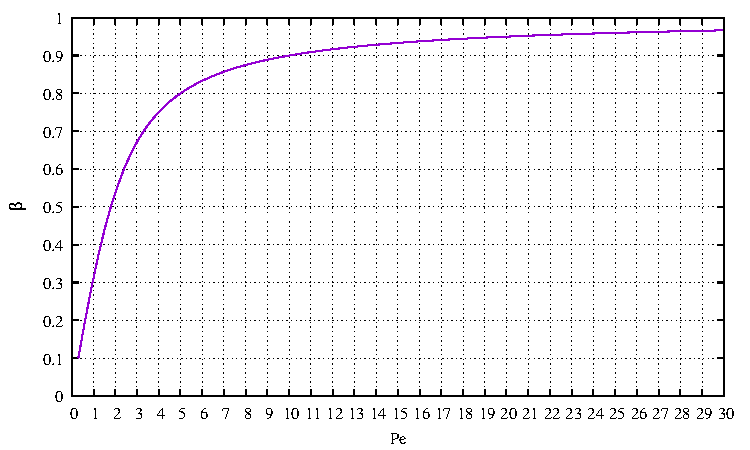
\includegraphics[width=10cm]{images/supg/beta1}
\end{center}


One can also define $\tilde{k}=\rho_0 C_p \tilde{\kappa}$ so that 
the discretised 1D advection-diffusion becomes:
\begin{equation}
\rho_0 C_p u \frac{T_{i+1}-T_{i-1}}{2h_x}
- (k+ \tilde{k}) \frac{T_{i-1}-2T_i+T_{i+1}}{h_x^2}
= f 
\end{equation}
or, in its continuous formulation:
\begin{eqnarray}
\rho_0 C_p u \frac{dT}{dx} - (k+ \tilde{k}) \frac{d^2T}{dx^2} &=& f \nn\\
\rho_0 C_p u \frac{dT}{dx}
- \tilde{k} \frac{d^2T}{dx^2} 
- k \frac{d^2T}{dx^2} &=& f \nn\\
\rho_0 C_p u \frac{dT}{dx}
- \rho_0 C_p \beta \frac{u h}{2} \frac{d^2T}{dx^2} 
- k \frac{d^2T}{dx^2} &=& f
\end{eqnarray}





%-----------------------------------------------------
\subsection{A note about linear elements - bubble functions \& Petrov-Galerkin formulation}

Let us assume that $u>0$, i.e. advection goes from left to right. 
Node $i-1$ is said to be on the upstream side of node $i$, and node $i+1$
is on the downstream side of node . In Petrov FEM, instead of selecting the weight functions to be the
same as the standard basis functions, we distort them as shown below.

\index{general}{Bubble Function}
The distortion is based on so-called bubble functions since they have zero
values on the nodes and they are nonzero on elements' interiors.
For instance one can take
\begin{eqnarray}
{\bN}^\star_1(r)&=&\frac{1}{2}(1-r)-\frac{3}{4}\beta(1-r^2) \\
{\bN}^\star_2(r)&=&\frac{1}{2}(1+r)+\frac{3}{4}\beta(1-r^2) 
\end{eqnarray}
as test/weight functions
where $\beta$ is a parameter that controls the amount of upwinding. 

The elemental advection matrix is then given by:
\begin{center}
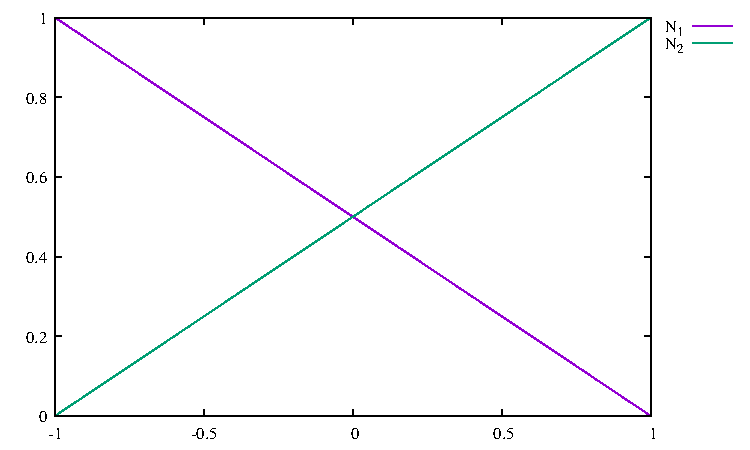
\includegraphics[width=6cm]{images/supg/bubble1}
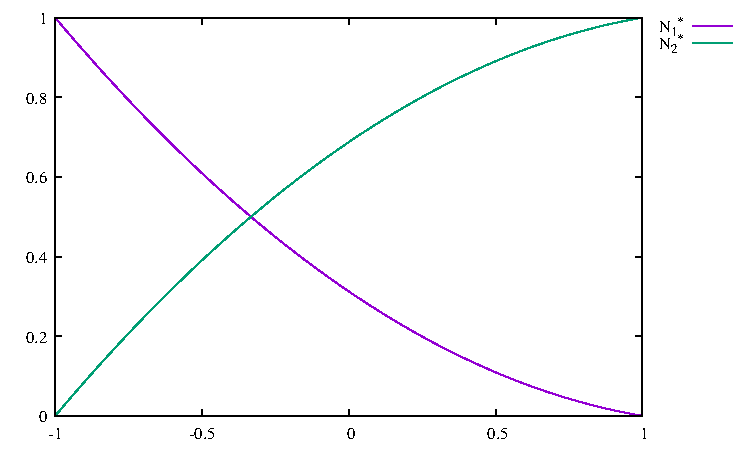
\includegraphics[width=6cm]{images/supg/bubble2}\\
{\captionfont Left: standard $Q_1$ test functions; Right: modified ($Q_1$+bubble) functions
for $\beta=0.25$}
\end{center}

\[
r = 2(x-x_k)/(x_{k+1}-x_{k}) -1 =2(x-x_k)/h  -1
\]
then 
\[
dr = \frac{2}{h} dx
\]
or
\[
dx=\frac{h}{2} dr
\]


\begin{eqnarray}
{\K}_a^e 
&=& \int_{x_k}^{x_{k+1}}   ({\vec \bN}^\star)^T \rho C_p \vec\upnu \cdot {\bm B} \; dx  \nn\\
&=& \frac{h}{2} \int_{-1}^{+1}   ({\vec \bN}^\star)^T \rho C_p \vec\upnu \cdot {\bm B} \; dr  \nn\\
&=& \frac{h}{2} \int_{-1}^{+1} 
\left(\begin{array}{c}
{\bN}_1^\star \\ {\bN}_2^\star 
\end{array}\right)
\rho C_p u \left( \frac{d\bN_1}{dr} \; \frac{d\bN_2}{dr} \right)  dr \nn\\
&=& 
\frac{h}{2} \rho C_p u \int_{-1}^{+1} 
\left(\begin{array}{c}
{\bN}_1 \\ {\bN}_2
\end{array}\right)
\left( \frac{d\bN_1}{dr} \; \frac{d\bN_2}{dr} \right)  dr
+
\frac{h}{2} \rho C_p u \int_{-1}^{+1} 
\left(\begin{array}{c}
-\frac{3}{4}\beta(1-r^2) \\ +\frac{3}{4}\beta(1-r^2) 
\end{array}\right)
\left( \frac{d\bN_1}{dr} \; \frac{d\bN_2}{dr} \right)  dr 
\nn\\
&=& 
\frac{h}{2} \rho C_p u \int_{-1}^{+1} 
\left(\begin{array}{c}
\frac12 (1-r) \\ \frac12(1+r)
\end{array}\right)
\left( -\frac12 \; \frac12 \right)  dr
+
\frac{h}{2} \rho C_p u \int_{-1}^{+1} 
\left(\begin{array}{c}
-\frac{3}{4}\beta(1-r^2) \\ +\frac{3}{4}\beta(1-r^2) 
\end{array}\right)
\left( -\frac12 \; \frac12 \right)  dr  
\nn\\
&=& \rho C_p u \frac{h}{8}\int_{-1}^{+1} 
\left(\begin{array}{cc}
-(1-r) & (1-r)  \\
-(1+r) & (1+r)
\end{array}\right)  dr
+
\frac{3h}{16}\beta
\rho C_p u \int_{-1}^{+1} 
\left(\begin{array}{cc}
(1-r^2) & -(1-r^2) \\
-(1-r^2) & (1-r^2) 
\end{array}\right)  dr
\nn\\
&=& \rho C_p u \frac{h}{8}
\left(\begin{array}{cc}
-2 & 2 \\
-2 & 2
\end{array}\right)  
+
\frac{3h}{16}\beta
\rho C_p u 
\left(\begin{array}{cc}
4/3 & -4/3 \\
-4/3 & 4/3 
\end{array}\right)   \nn\\
&=& \rho C_p u \frac{h}{4}
\left(\begin{array}{cc}
-1 & 1 \\
-1 & 1
\end{array}\right) 
+
\frac{h}{4}\beta
\rho C_p u 
\left(\begin{array}{cc}
1 & -1 \\
-1 & 1 
\end{array}\right)  
\end{eqnarray}
We see that this additional matrix is akin to ${\K}_d^e$ (albeit with a 
different diffusion coefficient).

